\documentclass[twoside]{book}

% Packages required by doxygen
\usepackage{fixltx2e}
\usepackage{calc}
\usepackage{doxygen}
\usepackage[export]{adjustbox} % also loads graphicx
\usepackage{graphicx}
\usepackage[utf8]{inputenc}
\usepackage{makeidx}
\usepackage{multicol}
\usepackage{multirow}
\PassOptionsToPackage{warn}{textcomp}
\usepackage{textcomp}
\usepackage[nointegrals]{wasysym}
\usepackage[table]{xcolor}

% Font selection
\usepackage[T1]{fontenc}
\usepackage[scaled=.90]{helvet}
\usepackage{courier}
\usepackage{amssymb}
\usepackage{sectsty}
\renewcommand{\familydefault}{\sfdefault}
\allsectionsfont{%
  \fontseries{bc}\selectfont%
  \color{darkgray}%
}
\renewcommand{\DoxyLabelFont}{%
  \fontseries{bc}\selectfont%
  \color{darkgray}%
}
\newcommand{\+}{\discretionary{\mbox{\scriptsize$\hookleftarrow$}}{}{}}

% Page & text layout
\usepackage{geometry}
\geometry{%
  a4paper,%
  top=2.5cm,%
  bottom=2.5cm,%
  left=2.5cm,%
  right=2.5cm%
}
\tolerance=750
\hfuzz=15pt
\hbadness=750
\setlength{\emergencystretch}{15pt}
\setlength{\parindent}{0cm}
\setlength{\parskip}{3ex plus 2ex minus 2ex}
\makeatletter
\renewcommand{\paragraph}{%
  \@startsection{paragraph}{4}{0ex}{-1.0ex}{1.0ex}{%
    \normalfont\normalsize\bfseries\SS@parafont%
  }%
}
\renewcommand{\subparagraph}{%
  \@startsection{subparagraph}{5}{0ex}{-1.0ex}{1.0ex}{%
    \normalfont\normalsize\bfseries\SS@subparafont%
  }%
}
\makeatother

% Headers & footers
\usepackage{fancyhdr}
\pagestyle{fancyplain}
\fancyhead[LE]{\fancyplain{}{\bfseries\thepage}}
\fancyhead[CE]{\fancyplain{}{}}
\fancyhead[RE]{\fancyplain{}{\bfseries\leftmark}}
\fancyhead[LO]{\fancyplain{}{\bfseries\rightmark}}
\fancyhead[CO]{\fancyplain{}{}}
\fancyhead[RO]{\fancyplain{}{\bfseries\thepage}}
\fancyfoot[LE]{\fancyplain{}{}}
\fancyfoot[CE]{\fancyplain{}{}}
\fancyfoot[RE]{\fancyplain{}{\bfseries\scriptsize Generated by Doxygen }}
\fancyfoot[LO]{\fancyplain{}{\bfseries\scriptsize Generated by Doxygen }}
\fancyfoot[CO]{\fancyplain{}{}}
\fancyfoot[RO]{\fancyplain{}{}}
\renewcommand{\footrulewidth}{0.4pt}
\renewcommand{\chaptermark}[1]{%
  \markboth{#1}{}%
}
\renewcommand{\sectionmark}[1]{%
  \markright{\thesection\ #1}%
}

% Indices & bibliography
\usepackage{natbib}
\usepackage[titles]{tocloft}
\setcounter{tocdepth}{3}
\setcounter{secnumdepth}{5}
\makeindex

% Hyperlinks (required, but should be loaded last)
\usepackage{ifpdf}
\ifpdf
  \usepackage[pdftex,pagebackref=true]{hyperref}
\else
  \usepackage[ps2pdf,pagebackref=true]{hyperref}
\fi
\hypersetup{%
  colorlinks=true,%
  linkcolor=blue,%
  citecolor=blue,%
  unicode%
}

% Custom commands
\newcommand{\clearemptydoublepage}{%
  \newpage{\pagestyle{empty}\cleardoublepage}%
}

\usepackage{caption}
\captionsetup{labelsep=space,justification=centering,font={bf},singlelinecheck=off,skip=4pt,position=top}

%===== C O N T E N T S =====

\begin{document}

% Titlepage & ToC
\hypersetup{pageanchor=false,
             bookmarksnumbered=true,
             pdfencoding=unicode
            }
\pagenumbering{alph}
\begin{titlepage}
\vspace*{7cm}
\begin{center}%
{\Large K\+P\+I-\/geometry }\\
\vspace*{1cm}
{\large Generated by Doxygen 1.8.13}\\
\end{center}
\end{titlepage}
\clearemptydoublepage
\pagenumbering{roman}
\tableofcontents
\clearemptydoublepage
\pagenumbering{arabic}
\hypersetup{pageanchor=true}

%--- Begin generated contents ---
\chapter{Hierarchical Index}
\section{Иерархия классов}
Иерархия классов.\begin{DoxyCompactList}
\item \contentsline{section}{t\+Vector\+:\+:Single\+Point\+Error}{\pageref{classtVector_1_1SinglePointError}}{}
\item \contentsline{section}{t\+Named}{\pageref{classtNamed}}{}
\begin{DoxyCompactList}
\item \contentsline{section}{t\+Line}{\pageref{classtLine}}{}
\item \contentsline{section}{t\+Plane}{\pageref{classtPlane}}{}
\item \contentsline{section}{t\+Point}{\pageref{classtPoint}}{}
\begin{DoxyCompactList}
\item \contentsline{section}{t\+Vector}{\pageref{classtVector}}{}
\end{DoxyCompactList}
\item \contentsline{section}{t\+Tetraedr}{\pageref{classtTetraedr}}{}
\item \contentsline{section}{t\+Triangle}{\pageref{classtTriangle}}{}
\end{DoxyCompactList}
\end{DoxyCompactList}

\chapter{Class Index}
\section{Классы}
Классы с их кратким описанием.\begin{DoxyCompactList}
\item\contentsline{section}{\hyperlink{classtVector_1_1SinglePointError}{t\+Vector\+::\+Single\+Point\+Error} \\*Класс ошибки, когда вектор задали двумя равными точками }{\pageref{classtVector_1_1SinglePointError}}{}
\item\contentsline{section}{\hyperlink{classtLine}{t\+Line} \\*Класс прямой линии }{\pageref{classtLine}}{}
\item\contentsline{section}{\hyperlink{classtNamed}{t\+Named} \\*Общий базовый класс для всех остальных классов }{\pageref{classtNamed}}{}
\item\contentsline{section}{\hyperlink{classtPlane}{t\+Plane} \\*Класс плоскости }{\pageref{classtPlane}}{}
\item\contentsline{section}{\hyperlink{classtPoint}{t\+Point} \\*Класс точки }{\pageref{classtPoint}}{}
\item\contentsline{section}{\hyperlink{classtTetraedr}{t\+Tetraedr} \\*Класс тетраэдра -\/ трегуольной пирамиды }{\pageref{classtTetraedr}}{}
\item\contentsline{section}{\hyperlink{classtTriangle}{t\+Triangle} \\*Класс треугольника }{\pageref{classtTriangle}}{}
\item\contentsline{section}{\hyperlink{classtVector}{t\+Vector} \\*Класс вектора }{\pageref{classtVector}}{}
\end{DoxyCompactList}

\chapter{Class Documentation}
\hypertarget{classtVector_1_1SinglePointError}{}\section{t\+Vector\+:\+:Single\+Point\+Error Class Reference}
\label{classtVector_1_1SinglePointError}\index{t\+Vector\+::\+Single\+Point\+Error@{t\+Vector\+::\+Single\+Point\+Error}}


Error class when the vector was set by two equal points.  




{\ttfamily \#include $<$geometry.\+hpp$>$}



\subsection{Detailed Description}
Error class when the vector was set by two equal points. 

The documentation for this class was generated from the following file\+:\begin{DoxyCompactItemize}
\item 
/home/b1zon/\+Desktop/cpp/\+K\+P\+I-\/geometrylib/include/geometry.\+hpp\end{DoxyCompactItemize}

\hypertarget{classtLine}{}\section{Класс t\+Line}
\label{classtLine}\index{t\+Line@{t\+Line}}


Класс прямой линии  




{\ttfamily \#include $<$russian\+\_\+version\+\_\+of\+\_\+geometry.\+hpp$>$}



Граф наследования\+:t\+Line\+:\nopagebreak
\begin{figure}[H]
\begin{center}
\leavevmode
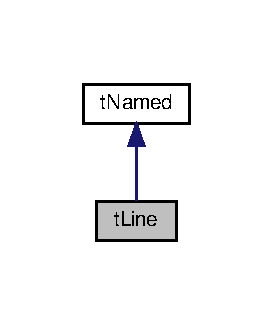
\includegraphics[width=131pt]{classtLine__inherit__graph}
\end{center}
\end{figure}


Граф связей класса t\+Line\+:\nopagebreak
\begin{figure}[H]
\begin{center}
\leavevmode
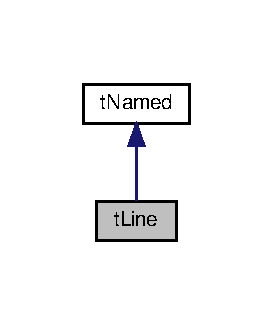
\includegraphics[width=131pt]{classtLine__coll__graph}
\end{center}
\end{figure}
\subsection*{Открытые члены}
\begin{DoxyCompactItemize}
\item 
\hyperlink{classtLine_ab61e326194db410630307c04cbbaf301}{t\+Line} (double newa=0, double newb=0, double newc=0, double newn=1, double newm=0, double newp=0, char const $\ast$New\+Name=\char`\"{}a Line\char`\"{})
\begin{DoxyCompactList}\small\item\em Конструктор через коефициенты  Уравнение прямой в пространстве\+: (x-\/a)/n = (x-\/b)/m = (x-\/c)/p. \end{DoxyCompactList}\item 
\mbox{\Hypertarget{classtLine_a8af9012ac69b257b296c9104a6f6fda7}\label{classtLine_a8af9012ac69b257b296c9104a6f6fda7}} 
\hyperlink{classtLine_a8af9012ac69b257b296c9104a6f6fda7}{t\+Line} (const \hyperlink{classtPoint}{t\+Point} \&A, const \hyperlink{classtPoint}{t\+Point} \&B, char const $\ast$New\+Name=\char`\"{}a Line\char`\"{})
\begin{DoxyCompactList}\small\item\em Конструктор через две точки и имя \end{DoxyCompactList}\item 
\mbox{\Hypertarget{classtLine_a5ee3acc8febba1e9f9473be6399341c8}\label{classtLine_a5ee3acc8febba1e9f9473be6399341c8}} 
\hyperlink{classtLine_a5ee3acc8febba1e9f9473be6399341c8}{t\+Line} (const \hyperlink{classtPoint}{t\+Point} \&S, const \hyperlink{classtVector}{t\+Vector} \&D, char const $\ast$New\+Name=\char`\"{}a Line\char`\"{})
\begin{DoxyCompactList}\small\item\em Конструктор через точку, вектор направления и имя \end{DoxyCompactList}\item 
\mbox{\Hypertarget{classtLine_a9a1dbb658383a93138ed00d8893c590b}\label{classtLine_a9a1dbb658383a93138ed00d8893c590b}} 
\hyperlink{classtLine_a9a1dbb658383a93138ed00d8893c590b}{t\+Line} (const \hyperlink{classtPlane}{t\+Plane} \&v1, const \hyperlink{classtPlane}{t\+Plane} \&v2, char const $\ast$New\+Name=\char`\"{}a Line\char`\"{})
\begin{DoxyCompactList}\small\item\em Конструктор чере пересечение двух плоскостей и имя \end{DoxyCompactList}\item 
\mbox{\Hypertarget{classtLine_a2154dba6e6089dcbb6c3a61a10bb76c1}\label{classtLine_a2154dba6e6089dcbb6c3a61a10bb76c1}} 
{\bfseries t\+Line} (const \hyperlink{classtLine}{t\+Line} \&)
\item 
\mbox{\Hypertarget{classtLine_a42c5470a9e40032639b6f22c82f90d9d}\label{classtLine_a42c5470a9e40032639b6f22c82f90d9d}} 
\hyperlink{classtLine_a42c5470a9e40032639b6f22c82f90d9d}{t\+Line} (const \hyperlink{classtPoint}{t\+Point} \&, const \hyperlink{classtPlane}{t\+Plane} \&)
\begin{DoxyCompactList}\small\item\em Конструктор прямой как перпендикуляр точки к плоскости \end{DoxyCompactList}\item 
\mbox{\Hypertarget{classtLine_ad74c8cba60f8719f6cfaaf7bb86933bc}\label{classtLine_ad74c8cba60f8719f6cfaaf7bb86933bc}} 
void \hyperlink{classtLine_ad74c8cba60f8719f6cfaaf7bb86933bc}{setnew} (double, double, double, double, double, double)
\begin{DoxyCompactList}\small\item\em Установить новые значения коефициентов \end{DoxyCompactList}\item 
bool \hyperlink{classtLine_aa824b319e4aa173d221ff28f55ec1890}{correct} () const
\item 
\mbox{\Hypertarget{classtLine_ae24e73371453cca328317f2512d9a53e}\label{classtLine_ae24e73371453cca328317f2512d9a53e}} 
\hyperlink{classtVector}{t\+Vector} \hyperlink{classtLine_ae24e73371453cca328317f2512d9a53e}{G\+Dir} () const
\begin{DoxyCompactList}\small\item\em Получить вектор направления \end{DoxyCompactList}\item 
\mbox{\Hypertarget{classtLine_aa2b2ab0dd465f2a824860b1f7211be1e}\label{classtLine_aa2b2ab0dd465f2a824860b1f7211be1e}} 
\hyperlink{classtPoint}{t\+Point} \hyperlink{classtLine_aa2b2ab0dd465f2a824860b1f7211be1e}{G\+Source} () const
\begin{DoxyCompactList}\small\item\em Получить начальную точку \end{DoxyCompactList}\item 
\mbox{\Hypertarget{classtLine_aab7ebec6bd8c0b93343b2410c96e4f72}\label{classtLine_aab7ebec6bd8c0b93343b2410c96e4f72}} 
double {\bfseries Sx} () const
\item 
\mbox{\Hypertarget{classtLine_a7d663774fd202f5aac5b7f8b2b0df4e7}\label{classtLine_a7d663774fd202f5aac5b7f8b2b0df4e7}} 
void {\bfseries Set\+Sx} (double)
\item 
\mbox{\Hypertarget{classtLine_a536f3e6c32bbfdf22d47db22c0d7c23e}\label{classtLine_a536f3e6c32bbfdf22d47db22c0d7c23e}} 
double {\bfseries Dx} () const
\item 
\mbox{\Hypertarget{classtLine_a3c927cf224e787e92d5738e203b14cdb}\label{classtLine_a3c927cf224e787e92d5738e203b14cdb}} 
void {\bfseries Set\+Dx} (double)
\item 
\mbox{\Hypertarget{classtLine_a7c99f5ee41a79b60d22e9484c13a30be}\label{classtLine_a7c99f5ee41a79b60d22e9484c13a30be}} 
double {\bfseries Sy} () const
\item 
\mbox{\Hypertarget{classtLine_a66b58812264146fe885327e0bc695908}\label{classtLine_a66b58812264146fe885327e0bc695908}} 
void {\bfseries Set\+Sy} (double)
\item 
\mbox{\Hypertarget{classtLine_a3bcd4c881b5a35c0a76c64994a7ef138}\label{classtLine_a3bcd4c881b5a35c0a76c64994a7ef138}} 
double {\bfseries Dy} () const
\item 
\mbox{\Hypertarget{classtLine_a89f21fd6ee1472f47100424b40e64706}\label{classtLine_a89f21fd6ee1472f47100424b40e64706}} 
void {\bfseries Set\+Dy} (double)
\item 
\mbox{\Hypertarget{classtLine_a22f561a20c77abe7ea6e842ca233001a}\label{classtLine_a22f561a20c77abe7ea6e842ca233001a}} 
double {\bfseries Sz} () const
\item 
\mbox{\Hypertarget{classtLine_afba2ee2d43b66b9bbbd955eb5183c7e9}\label{classtLine_afba2ee2d43b66b9bbbd955eb5183c7e9}} 
void {\bfseries Set\+Sz} (double)
\item 
\mbox{\Hypertarget{classtLine_abc6784d8434fcb7d7d9750da03e1c1dc}\label{classtLine_abc6784d8434fcb7d7d9750da03e1c1dc}} 
double {\bfseries Dz} () const
\item 
\mbox{\Hypertarget{classtLine_ae30c9e94b9bf36c5054f7a21ecc42495}\label{classtLine_ae30c9e94b9bf36c5054f7a21ecc42495}} 
void {\bfseries Set\+Dz} (double)
\item 
\mbox{\Hypertarget{classtLine_ac6a3f1c09cfbe241038e4e23ed223558}\label{classtLine_ac6a3f1c09cfbe241038e4e23ed223558}} 
void \hyperlink{classtLine_ac6a3f1c09cfbe241038e4e23ed223558}{Set\+Source} (const \hyperlink{classtPoint}{t\+Point} \&)
\begin{DoxyCompactList}\small\item\em Установить начальную точку \end{DoxyCompactList}\item 
\mbox{\Hypertarget{classtLine_acff75aa6563c398c06c2ed5e4d118bb4}\label{classtLine_acff75aa6563c398c06c2ed5e4d118bb4}} 
void \hyperlink{classtLine_acff75aa6563c398c06c2ed5e4d118bb4}{Set\+Dir} (const \hyperlink{classtVector}{t\+Vector} \&)
\begin{DoxyCompactList}\small\item\em Установить вектор направления \end{DoxyCompactList}\item 
\mbox{\Hypertarget{classtLine_aeab725824ab76aa77c24c909086647f7}\label{classtLine_aeab725824ab76aa77c24c909086647f7}} 
bool \hyperlink{classtLine_aeab725824ab76aa77c24c909086647f7}{Has\+Point} (const \hyperlink{classtPoint}{t\+Point} \&) const
\begin{DoxyCompactList}\small\item\em Проверить принадлежит ли точка прямой \end{DoxyCompactList}\item 
\mbox{\Hypertarget{classtLine_a5b0fe2c1ec1e51fdd35021ab37532ea8}\label{classtLine_a5b0fe2c1ec1e51fdd35021ab37532ea8}} 
double \hyperlink{classtLine_a5b0fe2c1ec1e51fdd35021ab37532ea8}{Dist\+To\+Point} (const \hyperlink{classtPoint}{t\+Point} \&) const
\begin{DoxyCompactList}\small\item\em Найти расстояние от точки к прямой \end{DoxyCompactList}\item 
\mbox{\Hypertarget{classtLine_a1c3671f6868050035c0b2e5c90eaa143}\label{classtLine_a1c3671f6868050035c0b2e5c90eaa143}} 
bool \hyperlink{classtLine_a1c3671f6868050035c0b2e5c90eaa143}{Line\+Par} (const \hyperlink{classtLine}{t\+Line} \&) const
\begin{DoxyCompactList}\small\item\em Проверить прямые на паралельность \end{DoxyCompactList}\item 
\mbox{\Hypertarget{classtLine_aca3e282559b32039c0aae22eaff100f6}\label{classtLine_aca3e282559b32039c0aae22eaff100f6}} 
\hyperlink{classtLine}{t\+Line} \& {\bfseries operator=} (const \hyperlink{classtLine}{t\+Line} \&)
\end{DoxyCompactItemize}
\subsection*{Друзья}
\begin{DoxyCompactItemize}
\item 
\mbox{\Hypertarget{classtLine_a39d9dbc55c19c2857c4d8fee4d25c667}\label{classtLine_a39d9dbc55c19c2857c4d8fee4d25c667}} 
bool {\bfseries operator==} (const \hyperlink{classtLine}{t\+Line} \&, const \hyperlink{classtLine}{t\+Line} \&)
\item 
\mbox{\Hypertarget{classtLine_a74399479e67eadce300f996b6ddf21c3}\label{classtLine_a74399479e67eadce300f996b6ddf21c3}} 
ostream \& {\bfseries operator$<$$<$} (ostream \&, const \hyperlink{classtLine}{t\+Line} \&)
\item 
\mbox{\Hypertarget{classtLine_a0f6f0d2af6275b58e63e6f5667bf587f}\label{classtLine_a0f6f0d2af6275b58e63e6f5667bf587f}} 
istream \& {\bfseries operator$>$$>$} (istream \&, \hyperlink{classtLine}{t\+Line} \&)
\end{DoxyCompactItemize}


\subsection{Подробное описание}
Класс прямой линии 

\subsection{Конструктор(ы)}
\mbox{\Hypertarget{classtLine_ab61e326194db410630307c04cbbaf301}\label{classtLine_ab61e326194db410630307c04cbbaf301}} 
\index{t\+Line@{t\+Line}!t\+Line@{t\+Line}}
\index{t\+Line@{t\+Line}!t\+Line@{t\+Line}}
\subsubsection{\texorpdfstring{t\+Line()}{tLine()}}
{\footnotesize\ttfamily t\+Line\+::t\+Line (\begin{DoxyParamCaption}\item[{double}]{newa = {\ttfamily 0},  }\item[{double}]{newb = {\ttfamily 0},  }\item[{double}]{newc = {\ttfamily 0},  }\item[{double}]{newn = {\ttfamily 1},  }\item[{double}]{newm = {\ttfamily 0},  }\item[{double}]{newp = {\ttfamily 0},  }\item[{char const $\ast$}]{New\+Name = {\ttfamily \char`\"{}a~Line\char`\"{}} }\end{DoxyParamCaption})}



Конструктор через коефициенты  Уравнение прямой в пространстве\+: (x-\/a)/n = (x-\/b)/m = (x-\/c)/p. 

Ввести коефициенты в таком порядке\+: a, b, c (сначала верхние), n, m, p (потом нижние) 

\subsection{Методы}
\mbox{\Hypertarget{classtLine_aa824b319e4aa173d221ff28f55ec1890}\label{classtLine_aa824b319e4aa173d221ff28f55ec1890}} 
\index{t\+Line@{t\+Line}!correct@{correct}}
\index{correct@{correct}!t\+Line@{t\+Line}}
\subsubsection{\texorpdfstring{correct()}{correct()}}
{\footnotesize\ttfamily bool t\+Line\+::correct (\begin{DoxyParamCaption}{ }\end{DoxyParamCaption}) const}

Проверить, не слишком ли малы коефициенты в уравнении (внутренняя функция) 

Объявления и описания членов класса находятся в файле\+:\begin{DoxyCompactItemize}
\item 
code/russian\+\_\+version\+\_\+of\+\_\+geometry.\+hpp\end{DoxyCompactItemize}

\hypertarget{classtNamed}{}\section{t\+Named Class Reference}
\label{classtNamed}\index{t\+Named@{t\+Named}}


Common base class for all other classes.  




{\ttfamily \#include $<$geometry.\+hpp$>$}



Inheritance diagram for t\+Named\+:
\nopagebreak
\begin{figure}[H]
\begin{center}
\leavevmode
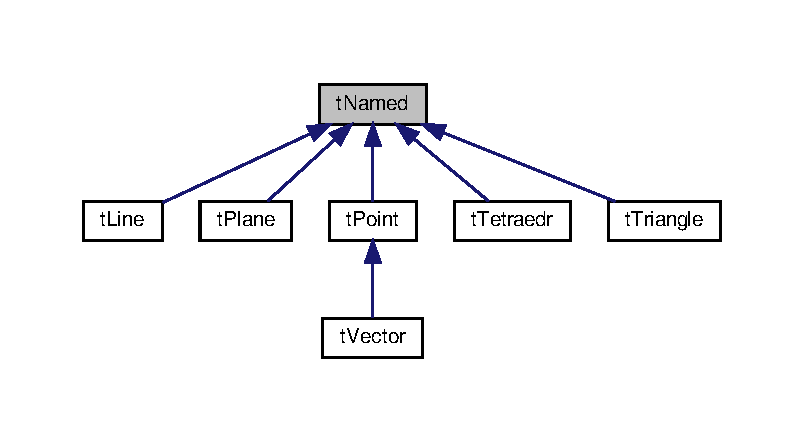
\includegraphics[width=350pt]{classtNamed__inherit__graph}
\end{center}
\end{figure}
\subsection*{Public Member Functions}
\begin{DoxyCompactItemize}
\item 
\mbox{\Hypertarget{classtNamed_a05e5161fa4d6de5530a35aebe379f99c}\label{classtNamed_a05e5161fa4d6de5530a35aebe379f99c}} 
\hyperlink{classtNamed_a05e5161fa4d6de5530a35aebe379f99c}{t\+Named} (char const $\ast$New\+Name=\char`\"{}\char`\"{})
\begin{DoxyCompactList}\small\item\em Constructor by name. \end{DoxyCompactList}\item 
\mbox{\Hypertarget{classtNamed_ab5f18adfba945ef9711b442680e7e613}\label{classtNamed_ab5f18adfba945ef9711b442680e7e613}} 
{\bfseries t\+Named} (const \hyperlink{classtNamed}{t\+Named} \&x)
\item 
\mbox{\Hypertarget{classtNamed_a8e159dc56389dad5e13d08097b1db3de}\label{classtNamed_a8e159dc56389dad5e13d08097b1db3de}} 
const char $\ast$ {\bfseries Name} () const
\item 
\mbox{\Hypertarget{classtNamed_a4ee0439b245fb018e39c3b3dd7e52d47}\label{classtNamed_a4ee0439b245fb018e39c3b3dd7e52d47}} 
char $\ast$ {\bfseries Name} ()
\item 
\mbox{\Hypertarget{classtNamed_a0f9ee5b68f19ab435fcdd263dd31c27f}\label{classtNamed_a0f9ee5b68f19ab435fcdd263dd31c27f}} 
int {\bfseries Name\+Length} () const
\item 
\mbox{\Hypertarget{classtNamed_a2cf8d7ca50e915fc1594b6a161f9334b}\label{classtNamed_a2cf8d7ca50e915fc1594b6a161f9334b}} 
\hyperlink{classtNamed}{t\+Named} \& {\bfseries operator=} (const \hyperlink{classtNamed}{t\+Named} \&)
\end{DoxyCompactItemize}


\subsection{Detailed Description}
Common base class for all other classes. 

The documentation for this class was generated from the following file\+:\begin{DoxyCompactItemize}
\item 
/home/b1zon/\+Desktop/cpp/\+K\+P\+I-\/geometrylib/include/geometry.\+hpp\end{DoxyCompactItemize}

\hypertarget{classtPlane}{}\section{t\+Plane Class Reference}
\label{classtPlane}\index{t\+Plane@{t\+Plane}}


Plane class.  




{\ttfamily \#include $<$geometry.\+hpp$>$}



Inheritance diagram for t\+Plane\+:
\nopagebreak
\begin{figure}[H]
\begin{center}
\leavevmode
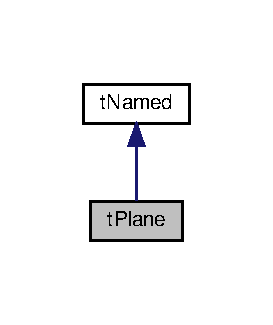
\includegraphics[width=131pt]{classtPlane__inherit__graph}
\end{center}
\end{figure}


Collaboration diagram for t\+Plane\+:
\nopagebreak
\begin{figure}[H]
\begin{center}
\leavevmode
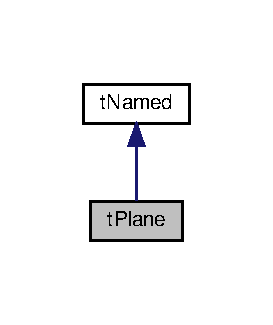
\includegraphics[width=131pt]{classtPlane__coll__graph}
\end{center}
\end{figure}
\subsection*{Public Member Functions}
\begin{DoxyCompactItemize}
\item 
\mbox{\Hypertarget{classtPlane_a82b8ca291bcb680731ea06067267bfe3}\label{classtPlane_a82b8ca291bcb680731ea06067267bfe3}} 
\hyperlink{classtPlane_a82b8ca291bcb680731ea06067267bfe3}{t\+Plane} (double newA=0, double newB=0, double newC=1, double newD=0, char const $\ast$New\+Name=\char`\"{}a Plane\char`\"{})
\begin{DoxyCompactList}\small\item\em Constructor by fields. \end{DoxyCompactList}\item 
\mbox{\Hypertarget{classtPlane_a18e2a0d542a83f8f250b70b9bda9c9c9}\label{classtPlane_a18e2a0d542a83f8f250b70b9bda9c9c9}} 
{\bfseries t\+Plane} (const \hyperlink{classtPlane}{t\+Plane} \&)
\item 
\mbox{\Hypertarget{classtPlane_a7232f7e46cd8e8ae4dfec128dd277b1f}\label{classtPlane_a7232f7e46cd8e8ae4dfec128dd277b1f}} 
\hyperlink{classtPlane_a7232f7e46cd8e8ae4dfec128dd277b1f}{t\+Plane} (const \hyperlink{classtPoint}{t\+Point} \&, const \hyperlink{classtPoint}{t\+Point} \&, const \hyperlink{classtPoint}{t\+Point} \&)
\begin{DoxyCompactList}\small\item\em Constructor by three points. \end{DoxyCompactList}\item 
\mbox{\Hypertarget{classtPlane_a4ddac807c5347da56a1300b7fb7b577f}\label{classtPlane_a4ddac807c5347da56a1300b7fb7b577f}} 
double {\bfseries A} () const
\item 
\mbox{\Hypertarget{classtPlane_a60ebb124c3ff083af76de458971844a6}\label{classtPlane_a60ebb124c3ff083af76de458971844a6}} 
void {\bfseries setA} (double)
\item 
\mbox{\Hypertarget{classtPlane_abf7d8f068035f46ca31c5da6566e7732}\label{classtPlane_abf7d8f068035f46ca31c5da6566e7732}} 
double {\bfseries B} () const
\item 
\mbox{\Hypertarget{classtPlane_ae6241f12630da93be209c38e1472119e}\label{classtPlane_ae6241f12630da93be209c38e1472119e}} 
void {\bfseries setB} (double)
\item 
\mbox{\Hypertarget{classtPlane_ac2a72791a7336b7c56afe1f5d396c52b}\label{classtPlane_ac2a72791a7336b7c56afe1f5d396c52b}} 
double {\bfseries C} () const
\item 
\mbox{\Hypertarget{classtPlane_a4ad41ca722a6da81d3758631f67db13b}\label{classtPlane_a4ad41ca722a6da81d3758631f67db13b}} 
void {\bfseries setC} (double)
\item 
\mbox{\Hypertarget{classtPlane_a962da3f8ce1289d44438ad8f7ffbbbfa}\label{classtPlane_a962da3f8ce1289d44438ad8f7ffbbbfa}} 
double {\bfseries D} () const
\item 
\mbox{\Hypertarget{classtPlane_aab58e6aa9e9e941a12d2aa5dd85cbc8c}\label{classtPlane_aab58e6aa9e9e941a12d2aa5dd85cbc8c}} 
void {\bfseries setD} (double)
\item 
\mbox{\Hypertarget{classtPlane_a21e7cda32a0a6111f92cb8102915d304}\label{classtPlane_a21e7cda32a0a6111f92cb8102915d304}} 
void \hyperlink{classtPlane_a21e7cda32a0a6111f92cb8102915d304}{setnew} (double, double, double, double)
\begin{DoxyCompactList}\small\item\em Set new fields values. \end{DoxyCompactList}\item 
bool \hyperlink{classtPlane_a382974c179a2bac3eb2da1d18c4dd860}{correct} () const
\item 
\mbox{\Hypertarget{classtPlane_a7891a14a7511d7526633be820ce1604d}\label{classtPlane_a7891a14a7511d7526633be820ce1604d}} 
void \hyperlink{classtPlane_a7891a14a7511d7526633be820ce1604d}{Normalize} ()
\begin{DoxyCompactList}\small\item\em Normalization of the plane. \end{DoxyCompactList}\item 
\hyperlink{classtPlane}{t\+Plane} \hyperlink{classtPlane_a8957e329f01270932a9a5b73ee9fe33a}{Normalize} () const
\item 
\mbox{\Hypertarget{classtPlane_a90727fd4cebd6ddb9a82482ad89a9edd}\label{classtPlane_a90727fd4cebd6ddb9a82482ad89a9edd}} 
bool \hyperlink{classtPlane_a90727fd4cebd6ddb9a82482ad89a9edd}{Has\+Point} (const \hyperlink{classtPoint}{t\+Point} \&) const
\begin{DoxyCompactList}\small\item\em Check whether the point is on the plane. \end{DoxyCompactList}\item 
\mbox{\Hypertarget{classtPlane_a08f5fac758dd76797e3571c76ec7b3fa}\label{classtPlane_a08f5fac758dd76797e3571c76ec7b3fa}} 
double \hyperlink{classtPlane_a08f5fac758dd76797e3571c76ec7b3fa}{Dist\+To\+Point} (const \hyperlink{classtPoint}{t\+Point} \&) const
\begin{DoxyCompactList}\small\item\em Find the distance from the point to the plane. \end{DoxyCompactList}\item 
\mbox{\Hypertarget{classtPlane_a90739f10ab1734192c38128f8b267c7f}\label{classtPlane_a90739f10ab1734192c38128f8b267c7f}} 
\hyperlink{classtPlane}{t\+Plane} \& {\bfseries operator=} (const \hyperlink{classtPlane}{t\+Plane} \&)
\end{DoxyCompactItemize}
\subsection*{Friends}
\begin{DoxyCompactItemize}
\item 
\mbox{\Hypertarget{classtPlane_a6451041e9d6964bdee537cfbbb12b661}\label{classtPlane_a6451041e9d6964bdee537cfbbb12b661}} 
bool {\bfseries operator==} (const \hyperlink{classtPlane}{t\+Plane} \&, const \hyperlink{classtPlane}{t\+Plane} \&)
\item 
\mbox{\Hypertarget{classtPlane_a17e0e9cf17cafb43cdcd42e043267101}\label{classtPlane_a17e0e9cf17cafb43cdcd42e043267101}} 
ostream \& {\bfseries operator$<$$<$} (ostream \&, const \hyperlink{classtPlane}{t\+Plane} \&)
\item 
\mbox{\Hypertarget{classtPlane_aee7595b1119f9dea39ba0c12dc8c4dc3}\label{classtPlane_aee7595b1119f9dea39ba0c12dc8c4dc3}} 
istream \& {\bfseries operator$>$$>$} (istream \&, \hyperlink{classtPlane}{t\+Plane} \&)
\end{DoxyCompactItemize}


\subsection{Detailed Description}
Plane class. 

\subsection{Member Function Documentation}
\mbox{\Hypertarget{classtPlane_a382974c179a2bac3eb2da1d18c4dd860}\label{classtPlane_a382974c179a2bac3eb2da1d18c4dd860}} 
\index{t\+Plane@{t\+Plane}!correct@{correct}}
\index{correct@{correct}!t\+Plane@{t\+Plane}}
\subsubsection{\texorpdfstring{correct()}{correct()}}
{\footnotesize\ttfamily bool t\+Plane\+::correct (\begin{DoxyParamCaption}{ }\end{DoxyParamCaption}) const}

Check if the coefficients in the equation are not too small (internal function) \mbox{\Hypertarget{classtPlane_a8957e329f01270932a9a5b73ee9fe33a}\label{classtPlane_a8957e329f01270932a9a5b73ee9fe33a}} 
\index{t\+Plane@{t\+Plane}!Normalize@{Normalize}}
\index{Normalize@{Normalize}!t\+Plane@{t\+Plane}}
\subsubsection{\texorpdfstring{Normalize()}{Normalize()}}
{\footnotesize\ttfamily \hyperlink{classtPlane}{t\+Plane} t\+Plane\+::\+Normalize (\begin{DoxyParamCaption}{ }\end{DoxyParamCaption}) const}

Normalization of the plane (for constant planes) \begin{DoxyReturn}{Returns}
normalized plane 
\end{DoxyReturn}


The documentation for this class was generated from the following file\+:\begin{DoxyCompactItemize}
\item 
/home/b1zon/\+Desktop/cpp/\+K\+P\+I-\/geometrylib/include/geometry.\+hpp\end{DoxyCompactItemize}

\hypertarget{classtPoint}{}\section{t\+Point Class Reference}
\label{classtPoint}\index{t\+Point@{t\+Point}}


Point class.  




{\ttfamily \#include $<$geometry.\+hpp$>$}



Inheritance diagram for t\+Point\+:
\nopagebreak
\begin{figure}[H]
\begin{center}
\leavevmode
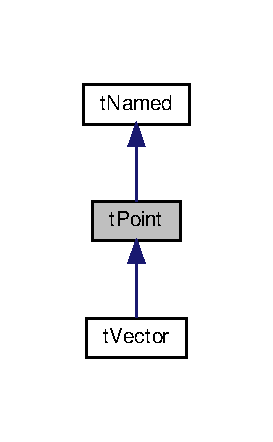
\includegraphics[width=131pt]{classtPoint__inherit__graph}
\end{center}
\end{figure}


Collaboration diagram for t\+Point\+:
\nopagebreak
\begin{figure}[H]
\begin{center}
\leavevmode
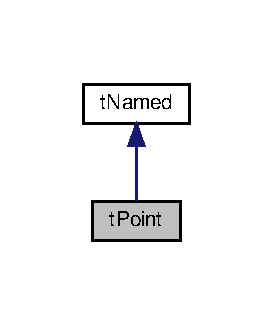
\includegraphics[width=131pt]{classtPoint__coll__graph}
\end{center}
\end{figure}
\subsection*{Public Member Functions}
\begin{DoxyCompactItemize}
\item 
\mbox{\Hypertarget{classtPoint_a0f7b95c63108ff1996f993f76208e4ee}\label{classtPoint_a0f7b95c63108ff1996f993f76208e4ee}} 
\hyperlink{classtPoint_a0f7b95c63108ff1996f993f76208e4ee}{t\+Point} (double newx=0, double newy=0, double newz=0, char const $\ast$New\+Name=\char`\"{}\char`\"{})
\begin{DoxyCompactList}\small\item\em Three point and name constructor. \end{DoxyCompactList}\item 
\mbox{\Hypertarget{classtPoint_acd4d6c37b06415e10f037c29eeeb35d2}\label{classtPoint_acd4d6c37b06415e10f037c29eeeb35d2}} 
{\bfseries t\+Point} (const \hyperlink{classtPoint}{t\+Point} \&)
\item 
\mbox{\Hypertarget{classtPoint_adfae7cc9253854321270b51acedcbc4d}\label{classtPoint_adfae7cc9253854321270b51acedcbc4d}} 
double {\bfseries x} () const
\item 
\mbox{\Hypertarget{classtPoint_ae7163ff0afe728da1be12f25844647e1}\label{classtPoint_ae7163ff0afe728da1be12f25844647e1}} 
void {\bfseries SetX} (double t)
\item 
\mbox{\Hypertarget{classtPoint_a3386f8a21f2f962327ee32b2f77f52ee}\label{classtPoint_a3386f8a21f2f962327ee32b2f77f52ee}} 
double {\bfseries y} () const
\item 
\mbox{\Hypertarget{classtPoint_ad9fb0cb6d30b24d7478a1d585fe4a491}\label{classtPoint_ad9fb0cb6d30b24d7478a1d585fe4a491}} 
void {\bfseries SetY} (double t)
\item 
\mbox{\Hypertarget{classtPoint_a14ad204b83379ad64b0c8ad6af6c4eab}\label{classtPoint_a14ad204b83379ad64b0c8ad6af6c4eab}} 
double {\bfseries z} () const
\item 
\mbox{\Hypertarget{classtPoint_a8da9a00e6d00624721b3dd9bb7a0df79}\label{classtPoint_a8da9a00e6d00624721b3dd9bb7a0df79}} 
void {\bfseries SetZ} (double t)
\item 
\mbox{\Hypertarget{classtPoint_ae712421b8ca24bf96a5516acaf773624}\label{classtPoint_ae712421b8ca24bf96a5516acaf773624}} 
double \hyperlink{classtPoint_ae712421b8ca24bf96a5516acaf773624}{Dist\+To} (const \hyperlink{classtPoint}{t\+Point} \&P) const
\begin{DoxyCompactList}\small\item\em Distance to another point. \end{DoxyCompactList}\item 
\mbox{\Hypertarget{classtPoint_ab85d062451a895276bcd60bdba888768}\label{classtPoint_ab85d062451a895276bcd60bdba888768}} 
void \hyperlink{classtPoint_ab85d062451a895276bcd60bdba888768}{Move} (const \hyperlink{classtPoint}{t\+Point} \&P)
\begin{DoxyCompactList}\small\item\em Move point. \end{DoxyCompactList}\item 
\mbox{\Hypertarget{classtPoint_a13e8f123791c52d15a9fc631ac47a7fe}\label{classtPoint_a13e8f123791c52d15a9fc631ac47a7fe}} 
void \hyperlink{classtPoint_a13e8f123791c52d15a9fc631ac47a7fe}{Turn\+X\+Point} (double phi)
\begin{DoxyCompactList}\small\item\em Rotate point in YoZ plane. \end{DoxyCompactList}\item 
\mbox{\Hypertarget{classtPoint_a7509d78eadd35f4e48da991927bab368}\label{classtPoint_a7509d78eadd35f4e48da991927bab368}} 
void \hyperlink{classtPoint_a7509d78eadd35f4e48da991927bab368}{Turn\+Y\+Point} (double phi)
\begin{DoxyCompactList}\small\item\em Rotate point in XoZ plane. \end{DoxyCompactList}\item 
\mbox{\Hypertarget{classtPoint_aea130545fd9a4a137901c483d2b9570f}\label{classtPoint_aea130545fd9a4a137901c483d2b9570f}} 
void \hyperlink{classtPoint_aea130545fd9a4a137901c483d2b9570f}{Turn\+Z\+Point} (double phi)
\begin{DoxyCompactList}\small\item\em Rotate a point in the XoY plane. \end{DoxyCompactList}\item 
\mbox{\Hypertarget{classtPoint_a01916af640294762c1946f10c03b06ec}\label{classtPoint_a01916af640294762c1946f10c03b06ec}} 
\hyperlink{classtPoint}{t\+Point} \& {\bfseries operator=} (const \hyperlink{classtPoint}{t\+Point} \&)
\end{DoxyCompactItemize}
\subsection*{Friends}
\begin{DoxyCompactItemize}
\item 
\mbox{\Hypertarget{classtPoint_a596f2f80bfe55efa7074306033e5656c}\label{classtPoint_a596f2f80bfe55efa7074306033e5656c}} 
bool {\bfseries operator==} (const \hyperlink{classtPoint}{t\+Point} \&, const \hyperlink{classtPoint}{t\+Point} \&)
\item 
\mbox{\Hypertarget{classtPoint_aca0717ecb2dfcd55c8b0a6eb56c6c16b}\label{classtPoint_aca0717ecb2dfcd55c8b0a6eb56c6c16b}} 
ostream \& {\bfseries operator$<$$<$} (ostream \&, const \hyperlink{classtPoint}{t\+Point} \&)
\item 
\mbox{\Hypertarget{classtPoint_a21e934e5bfe986e0b39885970a361047}\label{classtPoint_a21e934e5bfe986e0b39885970a361047}} 
istream \& {\bfseries operator$>$$>$} (istream \&, \hyperlink{classtPoint}{t\+Point} \&)
\end{DoxyCompactItemize}


\subsection{Detailed Description}
Point class. 

The documentation for this class was generated from the following file\+:\begin{DoxyCompactItemize}
\item 
/home/b1zon/\+Desktop/cpp/\+K\+P\+I-\/geometrylib/include/geometry.\+hpp\end{DoxyCompactItemize}

\hypertarget{classtTetraedr}{}\section{Класс t\+Tetraedr}
\label{classtTetraedr}\index{t\+Tetraedr@{t\+Tetraedr}}


Класс тетраэдра -\/ трегуольной пирамиды  




{\ttfamily \#include $<$russian\+\_\+version\+\_\+of\+\_\+geometry.\+hpp$>$}



Граф наследования\+:t\+Tetraedr\+:\nopagebreak
\begin{figure}[H]
\begin{center}
\leavevmode
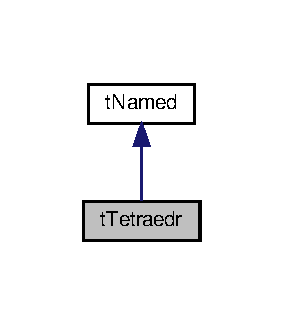
\includegraphics[width=136pt]{classtTetraedr__inherit__graph}
\end{center}
\end{figure}


Граф связей класса t\+Tetraedr\+:\nopagebreak
\begin{figure}[H]
\begin{center}
\leavevmode
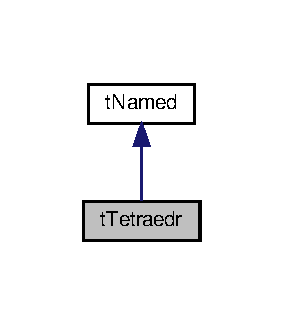
\includegraphics[width=136pt]{classtTetraedr__coll__graph}
\end{center}
\end{figure}
\subsection*{Открытые члены}
\begin{DoxyCompactItemize}
\item 
\mbox{\Hypertarget{classtTetraedr_ae16c310b01dbd8381503cf3610a9953e}\label{classtTetraedr_ae16c310b01dbd8381503cf3610a9953e}} 
\hyperlink{classtTetraedr_ae16c310b01dbd8381503cf3610a9953e}{t\+Tetraedr} (const \hyperlink{classtPoint}{t\+Point} \&V1, const \hyperlink{classtPoint}{t\+Point} \&V2, const \hyperlink{classtPoint}{t\+Point} \&V3, const \hyperlink{classtPoint}{t\+Point} \&S, char const $\ast$New\+Name=\char`\"{}a Tetraedr\char`\"{})
\begin{DoxyCompactList}\small\item\em Конструктор по четырем точкам и имени \end{DoxyCompactList}\item 
\mbox{\Hypertarget{classtTetraedr_ad276c51eebadada75b0e1a014421e426}\label{classtTetraedr_ad276c51eebadada75b0e1a014421e426}} 
\hyperlink{classtTetraedr_ad276c51eebadada75b0e1a014421e426}{t\+Tetraedr} (const \hyperlink{classtPlane}{t\+Plane} \&, const \hyperlink{classtPlane}{t\+Plane} \&, const \hyperlink{classtPlane}{t\+Plane} \&, const \hyperlink{classtPlane}{t\+Plane} \&, char const $\ast$New\+Name=\char`\"{}a Tetraedr\char`\"{})
\begin{DoxyCompactList}\small\item\em Конструктор по четырем плоскостям и имени \end{DoxyCompactList}\item 
\mbox{\Hypertarget{classtTetraedr_aef32a93d0050137e7bd1fff3688a830b}\label{classtTetraedr_aef32a93d0050137e7bd1fff3688a830b}} 
\hyperlink{classtTetraedr_aef32a93d0050137e7bd1fff3688a830b}{t\+Tetraedr} (const \hyperlink{classtTriangle}{t\+Triangle} \&, const \hyperlink{classtPoint}{t\+Point} \&, char const $\ast$New\+Name=\char`\"{}a Tetraedr\char`\"{})
\begin{DoxyCompactList}\small\item\em Конструктор по треугольнику(основе) и точке(четвертой вершине) и имени \end{DoxyCompactList}\item 
\mbox{\Hypertarget{classtTetraedr_a244165229504fe41e8ee386b6fdafc39}\label{classtTetraedr_a244165229504fe41e8ee386b6fdafc39}} 
\hyperlink{classtTetraedr_a244165229504fe41e8ee386b6fdafc39}{t\+Tetraedr} (double ax=0, double ay=0, double az=0, double bx=1, double by=0, double bz=0, double cx=0, double cy=1, double cz=0, double sx=0, double sy=0, double sz=1, char const $\ast$New\+Name=\char`\"{}a Tetraedr\char`\"{})
\begin{DoxyCompactList}\small\item\em Конструктор по координатам четырех точек и имени \end{DoxyCompactList}\item 
\mbox{\Hypertarget{classtTetraedr_afd21d86cdbebaf0cd0ce7ad2869a7011}\label{classtTetraedr_afd21d86cdbebaf0cd0ce7ad2869a7011}} 
{\bfseries t\+Tetraedr} (const \hyperlink{classtTetraedr}{t\+Tetraedr} \&)
\item 
bool \hyperlink{classtTetraedr_aa8b4ca43b819c0431fb28673b978d3c8}{correct} () const
\item 
\mbox{\Hypertarget{classtTetraedr_a897b074d2ee556801ba905e123a0f1e9}\label{classtTetraedr_a897b074d2ee556801ba905e123a0f1e9}} 
\hyperlink{classtPoint}{t\+Point} {\bfseries GetS} () const
\item 
\mbox{\Hypertarget{classtTetraedr_acd33af5079b8e6703b582144dca12b96}\label{classtTetraedr_acd33af5079b8e6703b582144dca12b96}} 
void {\bfseries SetS} (const \hyperlink{classtPoint}{t\+Point} \&)
\item 
\mbox{\Hypertarget{classtTetraedr_aab5ca30306a1915b174bcb6e248f4cae}\label{classtTetraedr_aab5ca30306a1915b174bcb6e248f4cae}} 
\hyperlink{classtTriangle}{t\+Triangle} {\bfseries GetT} () const
\item 
\mbox{\Hypertarget{classtTetraedr_aa7af31f49c73f7ec04cb350723ebfb40}\label{classtTetraedr_aa7af31f49c73f7ec04cb350723ebfb40}} 
void {\bfseries SetT} (const \hyperlink{classtTriangle}{t\+Triangle} \&)
\item 
\mbox{\Hypertarget{classtTetraedr_a7acaaa1f874fcff2d52a233297e96217}\label{classtTetraedr_a7acaaa1f874fcff2d52a233297e96217}} 
double \hyperlink{classtTetraedr_a7acaaa1f874fcff2d52a233297e96217}{Volume} () const
\begin{DoxyCompactList}\small\item\em Объём тетраэдра \end{DoxyCompactList}\item 
\mbox{\Hypertarget{classtTetraedr_a1460b237b37015925bb2da797574d364}\label{classtTetraedr_a1460b237b37015925bb2da797574d364}} 
\hyperlink{classtTetraedr}{t\+Tetraedr} \& {\bfseries operator=} (const \hyperlink{classtTetraedr}{t\+Tetraedr} \&)
\end{DoxyCompactItemize}
\subsection*{Друзья}
\begin{DoxyCompactItemize}
\item 
\mbox{\Hypertarget{classtTetraedr_a7d75847c4421b845c342d233964037c2}\label{classtTetraedr_a7d75847c4421b845c342d233964037c2}} 
bool {\bfseries operator==} (const \hyperlink{classtTetraedr}{t\+Tetraedr} \&, const \hyperlink{classtTetraedr}{t\+Tetraedr} \&)
\item 
\mbox{\Hypertarget{classtTetraedr_ad388d492e284583bda2df6567cb9ed83}\label{classtTetraedr_ad388d492e284583bda2df6567cb9ed83}} 
ostream \& {\bfseries operator$<$$<$} (ostream \&, const \hyperlink{classtTetraedr}{t\+Tetraedr} \&)
\item 
\mbox{\Hypertarget{classtTetraedr_a2d5eb752c4a11b1151046f7849146be0}\label{classtTetraedr_a2d5eb752c4a11b1151046f7849146be0}} 
istream \& {\bfseries operator$>$$>$} (istream \&, \hyperlink{classtTetraedr}{t\+Tetraedr} \&)
\end{DoxyCompactItemize}


\subsection{Подробное описание}
Класс тетраэдра -\/ трегуольной пирамиды 

\subsection{Методы}
\mbox{\Hypertarget{classtTetraedr_aa8b4ca43b819c0431fb28673b978d3c8}\label{classtTetraedr_aa8b4ca43b819c0431fb28673b978d3c8}} 
\index{t\+Tetraedr@{t\+Tetraedr}!correct@{correct}}
\index{correct@{correct}!t\+Tetraedr@{t\+Tetraedr}}
\subsubsection{\texorpdfstring{correct()}{correct()}}
{\footnotesize\ttfamily bool t\+Tetraedr\+::correct (\begin{DoxyParamCaption}{ }\end{DoxyParamCaption}) const}

Проверить, не слишком ли малы коефициенты в уравнении (внутренняя функция) 

Объявления и описания членов класса находятся в файле\+:\begin{DoxyCompactItemize}
\item 
code/russian\+\_\+version\+\_\+of\+\_\+geometry.\+hpp\end{DoxyCompactItemize}

\hypertarget{classtTriangle}{}\section{Класс t\+Triangle}
\label{classtTriangle}\index{t\+Triangle@{t\+Triangle}}


Класс треугольника  




{\ttfamily \#include $<$russian\+\_\+version\+\_\+of\+\_\+geometry.\+hpp$>$}



Граф наследования\+:t\+Triangle\+:\nopagebreak
\begin{figure}[H]
\begin{center}
\leavevmode
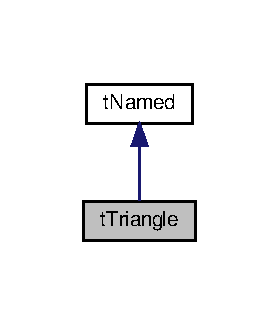
\includegraphics[width=134pt]{classtTriangle__inherit__graph}
\end{center}
\end{figure}


Граф связей класса t\+Triangle\+:\nopagebreak
\begin{figure}[H]
\begin{center}
\leavevmode
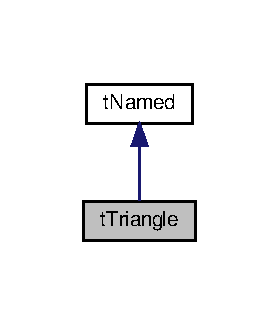
\includegraphics[width=134pt]{classtTriangle__coll__graph}
\end{center}
\end{figure}
\subsection*{Открытые члены}
\begin{DoxyCompactItemize}
\item 
\mbox{\Hypertarget{classtTriangle_a7d9deae65de86bc7dd8c4659921ab7e4}\label{classtTriangle_a7d9deae65de86bc7dd8c4659921ab7e4}} 
\hyperlink{classtTriangle_a7d9deae65de86bc7dd8c4659921ab7e4}{t\+Triangle} (double Ax=0, double Ay=0, double Az=0, double Bx=1, double By=0, double Bz=0, double Cx=0, double Cy=1, double Cz=0, char const $\ast$New\+Name=\char`\"{}a Triangle\char`\"{})
\begin{DoxyCompactList}\small\item\em Конструктор по координатам вершин и имени \end{DoxyCompactList}\item 
\mbox{\Hypertarget{classtTriangle_a083202f8a4ee5ad43997f7dfd02aa903}\label{classtTriangle_a083202f8a4ee5ad43997f7dfd02aa903}} 
\hyperlink{classtTriangle_a083202f8a4ee5ad43997f7dfd02aa903}{t\+Triangle} (const \hyperlink{classtPoint}{t\+Point} \&A, const \hyperlink{classtPoint}{t\+Point} \&B, const \hyperlink{classtPoint}{t\+Point} \&C, char const $\ast$New\+Name=\char`\"{}a Triangle\char`\"{})
\begin{DoxyCompactList}\small\item\em Конструктор по трем точкам(вершинам) \end{DoxyCompactList}\item 
\mbox{\Hypertarget{classtTriangle_a64a9bc79b605a895405862df622b2508}\label{classtTriangle_a64a9bc79b605a895405862df622b2508}} 
{\bfseries t\+Triangle} (const \hyperlink{classtTriangle}{t\+Triangle} \&T)
\item 
bool \hyperlink{classtTriangle_a21ecf9d970912497eca5009d6965aa54}{correct} () const
\item 
\mbox{\Hypertarget{classtTriangle_a75c20d7c45085d9d3b510c4a457c1daa}\label{classtTriangle_a75c20d7c45085d9d3b510c4a457c1daa}} 
\hyperlink{classtPoint}{t\+Point} {\bfseries GetA} () const
\item 
\mbox{\Hypertarget{classtTriangle_a2a6bbddf53b623165d2fba195287612b}\label{classtTriangle_a2a6bbddf53b623165d2fba195287612b}} 
void {\bfseries SetA} (const \hyperlink{classtPoint}{t\+Point} \&)
\item 
\mbox{\Hypertarget{classtTriangle_a243e7cc75b1a80d7a4901927d87c3161}\label{classtTriangle_a243e7cc75b1a80d7a4901927d87c3161}} 
\hyperlink{classtPoint}{t\+Point} {\bfseries GetB} () const
\item 
\mbox{\Hypertarget{classtTriangle_a6c694e33bc770411e93a43fd4066e198}\label{classtTriangle_a6c694e33bc770411e93a43fd4066e198}} 
void {\bfseries SetB} (const \hyperlink{classtPoint}{t\+Point} \&)
\item 
\mbox{\Hypertarget{classtTriangle_a1f282bae86e8a7c0e0d03c1daa1203cf}\label{classtTriangle_a1f282bae86e8a7c0e0d03c1daa1203cf}} 
\hyperlink{classtPoint}{t\+Point} {\bfseries GetC} () const
\item 
\mbox{\Hypertarget{classtTriangle_a918d25521066423811a5c8c6c065877d}\label{classtTriangle_a918d25521066423811a5c8c6c065877d}} 
void {\bfseries SetC} (const \hyperlink{classtPoint}{t\+Point} \&)
\item 
\mbox{\Hypertarget{classtTriangle_a97950f707d11df41c330fe3c9f87eefc}\label{classtTriangle_a97950f707d11df41c330fe3c9f87eefc}} 
double \hyperlink{classtTriangle_a97950f707d11df41c330fe3c9f87eefc}{Square} () const
\begin{DoxyCompactList}\small\item\em Найти площадь треугольника \end{DoxyCompactList}\item 
\mbox{\Hypertarget{classtTriangle_a130f7ecd50933a9dbcc1914fc4e31ac0}\label{classtTriangle_a130f7ecd50933a9dbcc1914fc4e31ac0}} 
\hyperlink{classtTriangle}{t\+Triangle} \& {\bfseries operator=} (const \hyperlink{classtTriangle}{t\+Triangle} \&)
\end{DoxyCompactItemize}
\subsection*{Друзья}
\begin{DoxyCompactItemize}
\item 
\mbox{\Hypertarget{classtTriangle_a95e318dd03b5dd2124a3b52fa6e5a398}\label{classtTriangle_a95e318dd03b5dd2124a3b52fa6e5a398}} 
bool {\bfseries operator==} (const \hyperlink{classtTriangle}{t\+Triangle} \&, const \hyperlink{classtTriangle}{t\+Triangle} \&)
\item 
\mbox{\Hypertarget{classtTriangle_a52e0f64418a864f97e0ef833d3c054c0}\label{classtTriangle_a52e0f64418a864f97e0ef833d3c054c0}} 
ostream \& {\bfseries operator$<$$<$} (ostream \&, const \hyperlink{classtTriangle}{t\+Triangle} \&)
\item 
\mbox{\Hypertarget{classtTriangle_a5b1b8bacb64f207e4d8c9bc5513c8335}\label{classtTriangle_a5b1b8bacb64f207e4d8c9bc5513c8335}} 
istream \& {\bfseries operator$>$$>$} (istream \&, \hyperlink{classtTriangle}{t\+Triangle} \&)
\end{DoxyCompactItemize}


\subsection{Подробное описание}
Класс треугольника 

\subsection{Методы}
\mbox{\Hypertarget{classtTriangle_a21ecf9d970912497eca5009d6965aa54}\label{classtTriangle_a21ecf9d970912497eca5009d6965aa54}} 
\index{t\+Triangle@{t\+Triangle}!correct@{correct}}
\index{correct@{correct}!t\+Triangle@{t\+Triangle}}
\subsubsection{\texorpdfstring{correct()}{correct()}}
{\footnotesize\ttfamily bool t\+Triangle\+::correct (\begin{DoxyParamCaption}{ }\end{DoxyParamCaption}) const}

Проверить, не слишком ли малы коефициенты в уравнении (внутренняя функция) 

Объявления и описания членов класса находятся в файле\+:\begin{DoxyCompactItemize}
\item 
code/russian\+\_\+version\+\_\+of\+\_\+geometry.\+hpp\end{DoxyCompactItemize}

\hypertarget{classtVector}{}\section{t\+Vector Class Reference}
\label{classtVector}\index{t\+Vector@{t\+Vector}}


Class vector.  




{\ttfamily \#include $<$geometry.\+hpp$>$}



Inheritance diagram for t\+Vector\+:
\nopagebreak
\begin{figure}[H]
\begin{center}
\leavevmode
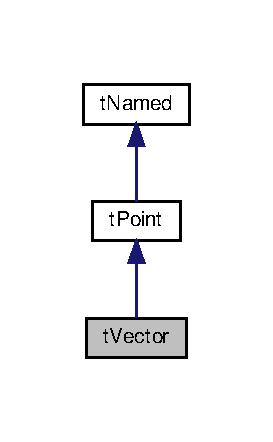
\includegraphics[width=131pt]{classtVector__inherit__graph}
\end{center}
\end{figure}


Collaboration diagram for t\+Vector\+:
\nopagebreak
\begin{figure}[H]
\begin{center}
\leavevmode
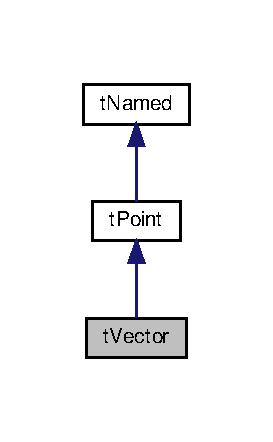
\includegraphics[width=131pt]{classtVector__coll__graph}
\end{center}
\end{figure}
\subsection*{Classes}
\begin{DoxyCompactItemize}
\item 
class \hyperlink{classtVector_1_1SinglePointError}{Single\+Point\+Error}
\begin{DoxyCompactList}\small\item\em Error class when the vector was set by two equal points. \end{DoxyCompactList}\end{DoxyCompactItemize}
\subsection*{Public Member Functions}
\begin{DoxyCompactItemize}
\item 
\mbox{\Hypertarget{classtVector_ad9dab835ddc33066445f3a00b77a0965}\label{classtVector_ad9dab835ddc33066445f3a00b77a0965}} 
\hyperlink{classtVector_ad9dab835ddc33066445f3a00b77a0965}{t\+Vector} (double newx, double newy, double newz, char const $\ast$New\+Name=\char`\"{}\char`\"{})
\begin{DoxyCompactList}\small\item\em Vector constructor via point coordinates (the first point is zero) \end{DoxyCompactList}\item 
\mbox{\Hypertarget{classtVector_aed3e3026b2483d748d4652cd3e79296d}\label{classtVector_aed3e3026b2483d748d4652cd3e79296d}} 
{\bfseries t\+Vector} (const \hyperlink{classtVector}{t\+Vector} \&)
\item 
\mbox{\Hypertarget{classtVector_a7dbffa8e340348bc896c578fd0335364}\label{classtVector_a7dbffa8e340348bc896c578fd0335364}} 
\hyperlink{classtVector_a7dbffa8e340348bc896c578fd0335364}{t\+Vector} (const \hyperlink{classtPoint}{t\+Point} \&, const \hyperlink{classtPoint}{t\+Point} \&)
\begin{DoxyCompactList}\small\item\em Vector by two points. \end{DoxyCompactList}\item 
\mbox{\Hypertarget{classtVector_a6573fc24ec1bfa80c6a5e21c1ea8be62}\label{classtVector_a6573fc24ec1bfa80c6a5e21c1ea8be62}} 
double \hyperlink{classtVector_a6573fc24ec1bfa80c6a5e21c1ea8be62}{Norm} () const
\begin{DoxyCompactList}\small\item\em Norm (length) of vector. \end{DoxyCompactList}\item 
\hyperlink{classtVector}{t\+Vector} \hyperlink{classtVector_a6141302c1bbad21b64e56d93ed0408e5}{Normalize} () const
\item 
\mbox{\Hypertarget{classtVector_a95d4d2975910e568033bd2a9d7df9c02}\label{classtVector_a95d4d2975910e568033bd2a9d7df9c02}} 
void \hyperlink{classtVector_a95d4d2975910e568033bd2a9d7df9c02}{Normalize} ()
\begin{DoxyCompactList}\small\item\em Normalization of a vector. \end{DoxyCompactList}\item 
\mbox{\Hypertarget{classtVector_accdeac1e568168edc72c3061f3f2c144}\label{classtVector_accdeac1e568168edc72c3061f3f2c144}} 
\hyperlink{classtVector}{t\+Vector} \& {\bfseries operator=} (const \hyperlink{classtVector}{t\+Vector} \&)
\item 
\mbox{\Hypertarget{classtVector_a15ace59ebe89a3d155a37dff222edfa0}\label{classtVector_a15ace59ebe89a3d155a37dff222edfa0}} 
\hyperlink{classtVector}{t\+Vector} \& {\bfseries operator$\ast$=} (double)
\item 
\mbox{\Hypertarget{classtVector_ace7606b4086cef0c8522a94f43c0ceb4}\label{classtVector_ace7606b4086cef0c8522a94f43c0ceb4}} 
\hyperlink{classtVector}{t\+Vector} \& {\bfseries operator+=} (const \hyperlink{classtVector}{t\+Vector} \&)
\item 
\mbox{\Hypertarget{classtVector_a81439447bad6a912c1e40be8ce5560bb}\label{classtVector_a81439447bad6a912c1e40be8ce5560bb}} 
\hyperlink{classtVector}{t\+Vector} \& {\bfseries operator-\/=} (const \hyperlink{classtVector}{t\+Vector} \&)
\item 
\mbox{\Hypertarget{classtVector_af49e6ba860ee5c38c66ae13f0c9c653f}\label{classtVector_af49e6ba860ee5c38c66ae13f0c9c653f}} 
\hyperlink{classtVector}{t\+Vector} \& {\bfseries operator$\ast$=} (const \hyperlink{classtVector}{t\+Vector} \&)
\end{DoxyCompactItemize}
\subsection*{Friends}
\begin{DoxyCompactItemize}
\item 
\mbox{\Hypertarget{classtVector_ac2deba186e1ddd047a218201d4cf1c6f}\label{classtVector_ac2deba186e1ddd047a218201d4cf1c6f}} 
bool {\bfseries operator==} (const \hyperlink{classtVector}{t\+Vector} \&, const \hyperlink{classtVector}{t\+Vector} \&)
\item 
\mbox{\Hypertarget{classtVector_ade0381c9b2e5496022391703599e1cfe}\label{classtVector_ade0381c9b2e5496022391703599e1cfe}} 
\hyperlink{classtVector}{t\+Vector} \& \hyperlink{classtVector_ade0381c9b2e5496022391703599e1cfe}{operator$\ast$} (const \hyperlink{classtVector}{t\+Vector} \&, double)
\begin{DoxyCompactList}\small\item\em Scalar multiplication on the right. \end{DoxyCompactList}\item 
\mbox{\Hypertarget{classtVector_a64a031b3695b984a50c362f8127f5bea}\label{classtVector_a64a031b3695b984a50c362f8127f5bea}} 
\hyperlink{classtVector}{t\+Vector} \& {\bfseries operator$\ast$} (double, const \hyperlink{classtVector}{t\+Vector} \&)
\item 
\mbox{\Hypertarget{classtVector_a9915bc8041ae050a433e85aea90f5471}\label{classtVector_a9915bc8041ae050a433e85aea90f5471}} 
\hyperlink{classtVector}{t\+Vector} \& \hyperlink{classtVector_a9915bc8041ae050a433e85aea90f5471}{operator+} (const \hyperlink{classtVector}{t\+Vector} \&, const \hyperlink{classtVector}{t\+Vector} \&)
\begin{DoxyCompactList}\small\item\em Sum of vectors. \end{DoxyCompactList}\item 
\mbox{\Hypertarget{classtVector_ab805cb8e1108272d31808bf4d258ba15}\label{classtVector_ab805cb8e1108272d31808bf4d258ba15}} 
\hyperlink{classtVector}{t\+Vector} \& \hyperlink{classtVector_ab805cb8e1108272d31808bf4d258ba15}{operator-\/} (const \hyperlink{classtVector}{t\+Vector} \&, const \hyperlink{classtVector}{t\+Vector} \&)
\begin{DoxyCompactList}\small\item\em Vectors difference. \end{DoxyCompactList}\item 
\mbox{\Hypertarget{classtVector_abec310e2c4d30878d11d0b2f5d02cad4}\label{classtVector_abec310e2c4d30878d11d0b2f5d02cad4}} 
\hyperlink{classtVector}{t\+Vector} \& \hyperlink{classtVector_abec310e2c4d30878d11d0b2f5d02cad4}{operator$\ast$} (const \hyperlink{classtVector}{t\+Vector} \&, const \hyperlink{classtVector}{t\+Vector} \&)
\begin{DoxyCompactList}\small\item\em Vector product of vectors. \end{DoxyCompactList}\item 
\mbox{\Hypertarget{classtVector_afcc0074f806c5d4f45eb32158292ca8c}\label{classtVector_afcc0074f806c5d4f45eb32158292ca8c}} 
ostream \& {\bfseries operator$<$$<$} (ostream \&, const \hyperlink{classtVector}{t\+Vector} \&)
\item 
\mbox{\Hypertarget{classtVector_a40b256a9f985011f794517f158deffe5}\label{classtVector_a40b256a9f985011f794517f158deffe5}} 
istream \& {\bfseries operator$>$$>$} (istream \&, \hyperlink{classtVector}{t\+Vector} \&)
\item 
\mbox{\Hypertarget{classtVector_a79cac88f76447395991d4dde1f173bfa}\label{classtVector_a79cac88f76447395991d4dde1f173bfa}} 
double \hyperlink{classtVector_a79cac88f76447395991d4dde1f173bfa}{operator,} (const \hyperlink{classtVector}{t\+Vector} \&, const \hyperlink{classtVector}{t\+Vector} \&)
\begin{DoxyCompactList}\small\item\em Dot product of vectors. \end{DoxyCompactList}\end{DoxyCompactItemize}


\subsection{Detailed Description}
Class vector. 

\subsection{Member Function Documentation}
\mbox{\Hypertarget{classtVector_a6141302c1bbad21b64e56d93ed0408e5}\label{classtVector_a6141302c1bbad21b64e56d93ed0408e5}} 
\index{t\+Vector@{t\+Vector}!Normalize@{Normalize}}
\index{Normalize@{Normalize}!t\+Vector@{t\+Vector}}
\subsubsection{\texorpdfstring{Normalize()}{Normalize()}}
{\footnotesize\ttfamily \hyperlink{classtVector}{t\+Vector} t\+Vector\+::\+Normalize (\begin{DoxyParamCaption}{ }\end{DoxyParamCaption}) const}

Normalization of a vector (for constant vectors) \begin{DoxyReturn}{Returns}
normalized vector 
\end{DoxyReturn}


The documentation for this class was generated from the following file\+:\begin{DoxyCompactItemize}
\item 
/home/b1zon/\+Desktop/cpp/\+K\+P\+I-\/geometrylib/include/geometry.\+hpp\end{DoxyCompactItemize}

%--- End generated contents ---

% Index
\backmatter
\newpage
\phantomsection
\clearemptydoublepage
\addcontentsline{toc}{chapter}{Index}
\printindex

\end{document}
